%Dokumentklasse
\documentclass[a4paper,12pt,makeidx,
twoside,
openright,
numbers=noenddot]{scrreprt}
\usepackage[left=3cm, right=2cm, bottom=2.5cm, top=3cm]{geometry}		% Formatierung der Seitenränder
%\usepackage[onehalfspacing]{setspace}							% verwendet für größeren Zeilenabstand

% ============= Packages =============

% Dokumentinformationen
\usepackage[
	pdftitle={},
	pdfsubject={},
	pdfauthor={},
	pdfkeywords={},
	%Links nicht einrahmen
	hidelinks
]{hyperref}

\usepackage[utf8]{inputenc}
\usepackage[ngerman]{babel}
\usepackage[T1]{fontenc}
\usepackage{units}
\usepackage{pdfpages}
\usepackage{listings}
\usepackage{svg}					% Zur Einbindung von scalable vector graphics
\usepackage{subcaption}				% Zum Einbinden von Untergrafiken
\usepackage[gen]{eurosym}			% Zur Verwendung des Eurozeichens
\usepackage{amssymb}
\usepackage{graphicx}
\graphicspath{{img/}}				
\usepackage{fancyhdr}				% Style Package für's Seitenlayout
\usepackage{color}					% anpassen von Farben
\usepackage{microtype} 				% schönerer Blocksatz!
\usepackage{calc}  					
\usepackage{enumitem}				% zb für align der description
\usepackage[font=small,labelfont=bf]{caption}
\usepackage[printonlyused]{acronym}	% für Abkürzungen
\usepackage{multicol}
\usepackage{booktabs}
\usepackage{textcomp}
\usepackage{listings}				% Einbindung von Code in LateX
\usepackage{setspace}
\usepackage{threeparttable} 		% für Fußnoten innerhalb einer Tabelle


% verschiedene Schriftarten
%\usepackage{times} 				% times font
%\usepackage{palatino}			 	% Palatino font
\usepackage{lmodern}				% Lmodern sans und serif
%\usepackage{libertine}				% Linux Libertine und Biolinum

%\usepackage{fontspec}				% Nutzen in Kombination mit LuaLaTeX, um Systemschriften einzubinden
%\setmainfont{Georgia}				% beispielsweise Georgia, aber auch jede andere Schrift, die auf dem PC vorhanden ist


% zusätzliche Schriftzeichen der American Mathematical Society
\usepackage{amsfonts}
\usepackage{amsmath}

\usepackage[numbers, comma]{natbib}		% Einstellung des Zitierstils
\bibliographystyle{myabbrvnat}			% Angepasster Stil für deutsche Sprache

\setcounter{secnumdepth}{3}				% Nummerierungsebene anpassen -> 3 = subsubsection werden nummeriert
\setcounter{tocdepth}{1}   				% gliederungsebenen im Inhaltsverzeichnis -> erstmal nur zur übersicht was nicht vergessen werden darf

\definecolor{deepblue}{rgb}{0,0,0.5}
\definecolor{deepred}{rgb}{0.6,0,0}
\definecolor{deepgreen}{rgb}{0,0.5,0}


% ============= Kopf- und Fußzeile =============
\pagestyle{fancy}

%% Formatierung der Kopf- und Fußzeile
\fancyhead{}
\fancyhead[RO,LE]{\thepage}
\fancyhead[RE]{\leftmark}
\fancyhead[LO]{\rightmark}
%%
\fancyfoot{}

\renewcommand{\headrulewidth}{0.4pt}		% Bei zweiseitigem Dokument ausschließlich Linie in Kopfzeile
\renewcommand{\chaptermark}[1]{\markboth{\thechapter\ #1}{}}
\renewcommand{\sectionmark}[1]{\markright{\thesection\ #1}}

% ============= Package Einstellungen & Sonstiges ============= 
% Besondere Trennungen
\hyphenation{Um-ge-bungs-tem-pe-ra-tur Um-ge-bungs-tem-pe-ra-tur-en Rauch-gas-tem-pe-ra-tur Aus-tritts-tem-pe-ra-tur}

% Einstellung wie Code innerhalb der Arbeit gesetzt werden soll:
\lstdefinestyle{Style}{
	columns=flexible,
	basicstyle=\ttfamily}
\lstset{ 
	backgroundcolor=\color{white},   % choose the background color; you must add \usepackage{color} or \usepackage{xcolor}; should come as last argument
	basicstyle=\footnotesize,        % the size of the fonts that are used for the code
	breakatwhitespace=false,         % sets if automatic breaks should only happen at whitespace
	breaklines=true,                 % sets automatic line breaking
	captionpos=none,                 % sets the caption-position to bottom
	commentstyle=\color{deepblue},   % comment style
	deletekeywords={...},            % if you want to delete keywords from the given language
	escapeinside={\%*}{*)},          % if you want to add LaTeX within your code
	extendedchars=true,              % lets you use non-ASCII characters; for 8-bits encodings only, does not work with UTF-8
	firstnumber=1,               	 % start line enumeration with line 1000
	frame=single,	                 % adds a frame around the code
	keepspaces=true,                 % keeps spaces in text, useful for keeping indentation of code (possibly needs columns=flexible)
	keywordstyle=\color{blue},       % keyword style
	language=Python,                 % the language of the code
	morekeywords={*,...},            % if you want to add more keywords to the set
	numbers=left,                    % where to put the line-numbers; possible values are (none, left, right)
	numbersep=5pt,                   % how far the line-numbers are from the code
	emphstyle=\color{deepred},
	%numberstyle=\tiny\color{mygray}, % the style that is used for the line-numbers
	rulecolor=\color{black},         % if not set, the frame-color may be changed on line-breaks within not-black text (e.g. comments (green here))
	showspaces=false,                % show spaces everywhere adding particular underscores; it overrides 'showstringspaces'
	showstringspaces=false,          % underline spaces within strings only
	showtabs=false,                  % show tabs within strings adding particular underscores
	stepnumber=2,                    % the step between two line-numbers. If it's 1, each line will be numbered
	stringstyle=\color{deepgreen},     % string literal style
	tabsize=2,	                   	 % sets default tabsize to 2 spaces
	title=\lstname                   % show the filename of files included with \lstinputlisting; also try caption instead of title
}

% nicht einrücken nach Absatz
\setlength{\parindent}{0pt}
\usepackage{parskip}		 			% verhindert einrücken und setzt einen kleinen Absatz

\renewcommand{\arraystretch}{1.2}		% Abstand innerhalb der Tabellen einstellen

% ============= Dokumentbeginn =============

\begin{document}
	
% Seiten ohne Kopf- und Fußzeile sowie Seitenzahl
\pagestyle{empty}

\begin{center}
\begin{tabular}{p{\textwidth}}

\begin{center}
	
\includegraphics[scale=0.35]{img/logos.jpg}
\end{center}


\\

\begin{center}
\LARGE{\textbf{
\LaTeX-Vorlage für Berichte, Bachelor- oder Masterarbeiten\\[1cm]
}}
\end{center}

\\


\begin{center}
\large{Hochschule Flensburg\\
Fachbereich 1: \textit{Musterstudiengang}\\}
\end{center}

\\\\

\begin{center}
\textbf{\Large{Abschlussarbeit}}
\end{center}


\begin{center}
zur Erlangung des akademischen Grades\\
Master of Engineering
\end{center}

\\\\

\begin{center}
vorgelegt von
\end{center}

\begin{center}
\large{\textbf{Max Mustermann}} \\
% \small{geboren am 01.01.0001 in Entenhausen}
\end{center}

\begin{center}
\large{\today}
\end{center}

\\
\\
\\

\begin{center}
\begin{tabular}{lll}
\textbf{Erstprüfer:} & & Prof. Dr.-Ing. Max Mustermann\\
\textbf{Zweitprüfer:} & & Prof. Dr.-Ing. Maxima Musterfrau\\
\end{tabular}
\end{center}

\end{tabular}
\end{center}		% Einbinden der Titelseite
\newpage 					% Um Seite nach der Titelseite einzubinden -> bei eigener Tittelseite und nicht der Latex-Version erforderlich
\thispagestyle{empty}
\quad 
\newpage
\pagenumbering{Roman}
 
\cleardoubleoddpage


\chapter*{Eidesstattliche Erklärung}
Ich versichere, dass ich die vorliegende Thesis ohne fremde Hilfe selbstständig verfasst und nur die angegebenen Quellen benutzt habe. \\~\\
Flensburg, den \today\\[.6cm]
Max Mustermann\\
\rule[0.5em]{20em}{0.5pt}

\chapter*{Zusammenfassung}

Diese \LaTeX-Vorlage ist für Berichte, Bachelor- sowie Masterarbeiten gedacht. Natürlich ist sie nicht perfekt und jede Art der Verbesserung wird dankend angenommen. Bei Fragen zur Verwendung oder Anregungen zur Verbesserung können Sie mir diese gern an markus.brandt1992@gmail.com senden.

An entsprechender Stelle werden Beispiele für die Verwendung von Abkürzungen, Zitaten, Abbildungen, Tabellen und die Einbettung von Code gegeben.



\tableofcontents			%Inhaltsverzeichnis
\listoffigures				%Verzeichnis aller Bilder
\listoftables				%Verzeichnis aller Tabellen
\chapter*{Abkürzungsverzeichnis}
	\begin{acronym}[4GDH]	% Zur Formatierung hier die längste Abkürzung des Verzeichnisses eintragen
		\acro{4GDH}{4th Generation District Heating} 	
	\end{acronym}

\pagestyle{fancy}

\chapter{Einleitung}
\pagenumbering{arabic}
	\section{Hintergrund}
	
	\section{Methodik}
	
	\section{Stand der Wissenschaft}


\chapter{Grundlagen}\label{chapter: Grundlagen}	

	\section{Abkürzungen}
	Abkürzungen im Text lassen sich mit dem Paket \textit{acronym} verwenden:\\ 
	\ac{4GDH}\\ 
	Bei der nächsten Verwendung im Text wird dann nur noch die Abkürzung verwendet \ac{4GDH}
	
	
	\section{Quellenangaben}
	Nach \citet{WINTERSCHEID2017579} kann angenommen werden, dass ...
	
	Energie besteht aus Exergie und Anergie \cite{Baehr2012}.
	
	
	\section{Abbildungen}
	In Abbildung \ref{fig: Abbildung X} ist zu erkennen, dass ... 
	\begin{figure}[ht]
		\begin{subfigure}[b]{0.49\textwidth}
			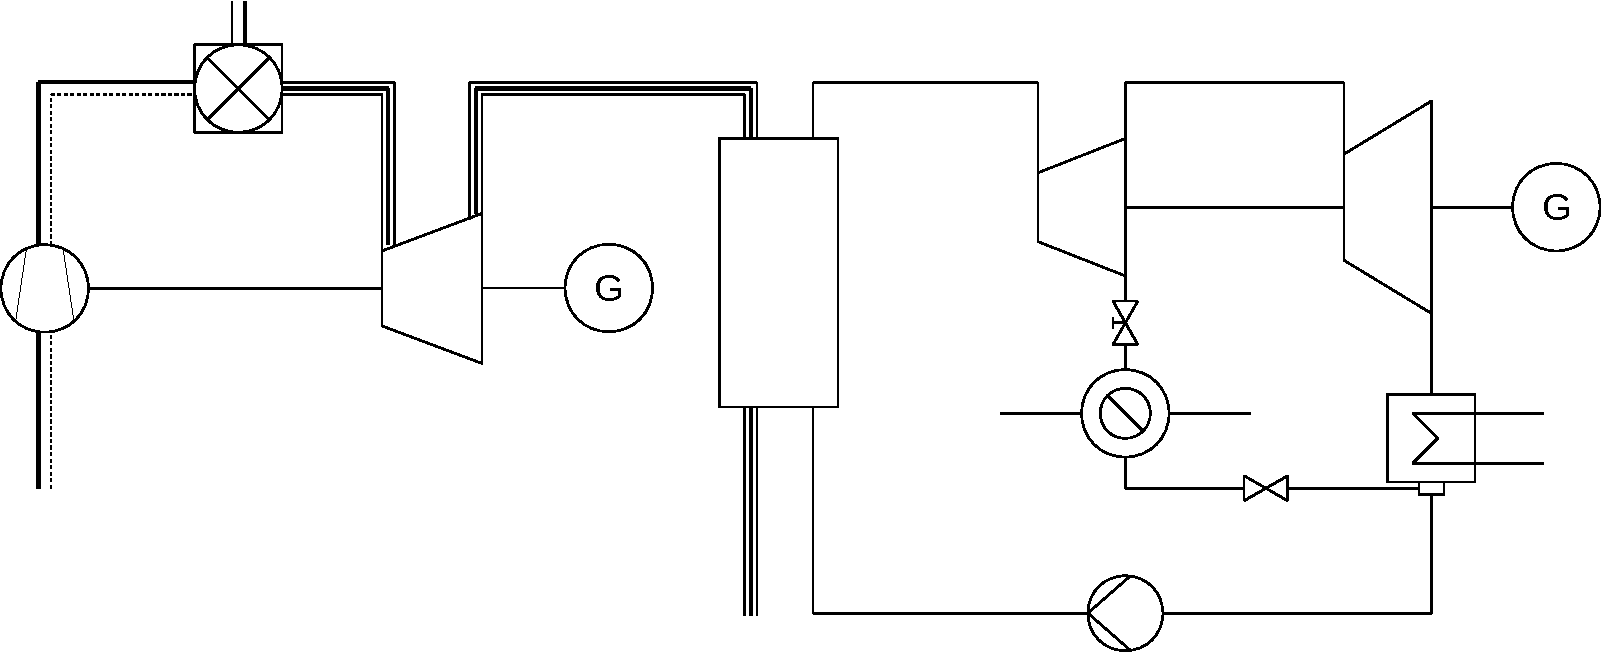
\includegraphics[width=1\textwidth]{SchaltplanGuD.pdf}
			\subcaption{Gas- und Dampfkraftwerk}
			\label{subfigure: Schaltplan_GuD}
		\end{subfigure}
		\hfill
		\begin{subfigure}[b]{0.49\textwidth}
			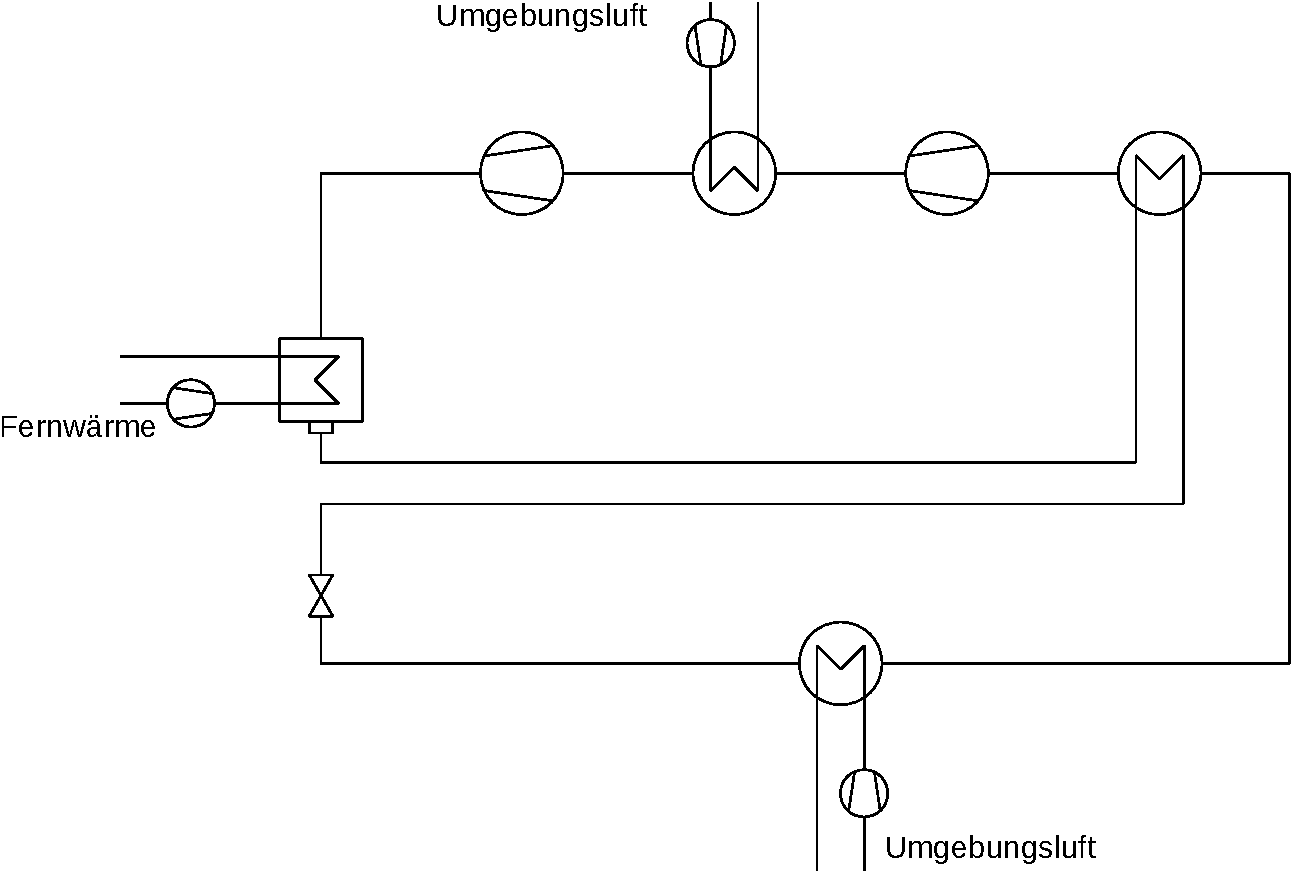
\includegraphics[width=1\textwidth]{Heatpump.pdf}
			\subcaption{Wärmepumpe}
			\label{subfigure: Schaltbild_Heatpump}
		\end{subfigure}
		\caption[Gegenüberstellung Gas- und Dampfkraftwerk mit Wärmepumpe]{Abbildung \ref{subfigure: Schaltplan_GuD} zeigt das Wärmeschaltbild eines Gas- und Dampfkraftwerks mit einer einfachen Entnahme im Dampfturbinen Teil. Abbildung \ref{subfigure: Schaltbild_Heatpump} zeigt hingegen das Schaltbild einer Kompressionswärmepumpe mit einfacher Kondensatunterkühlung.}
		\label{fig: Abbildung X}
	\end{figure}
	
	
	\section{Tabellen}
	Hinzufügen von Fußnoten innerhalb der Tabelle können zusätzliche Informationen zu bestimmten Werten oder Bezeichnungen gegeben werden - in diesem Fall, dass die angegebene Grädigkeit für alle Wärmeübertrager gilt.
    	\begin{center}
    	    \captionof{table}{Auslegungsparameter des Gas- und Dampfkraftwerks}
    		\begin{threeparttable}
        		\begin{tabular}{lllll}
        			\hline 
        			Teilprozess & Parameter  & Symbol  & Einheit  & Wert\tabularnewline
        			\hline 
        			\textbf{Fernwärme} & Vorlauftemperatur  & $T_{\text{VL}}$  & \textdegree C  &  124\tabularnewline
        			& Rücklauftemperatur  & $T_{\text{RL}}$  & \textdegree C  & 50\tabularnewline
        			& Druck  & $p_{\text{FW}}$  & bar  & 10\tabularnewline
        			& Wärmeaufnahme & $\dot{Q}_\text{DH}$ & MW & 145 \tabularnewline
        			\textbf{Gasturbinenprozess} & Brennstoffmassenstrom  & $\dot{m}_{\text{Fuel}}$  & kg/s  & 11,58 \tabularnewline
        			& Umgebungstemperatur  & $T_{\text{U}}$  & \textdegree C & 20 \tabularnewline
        			& Verbrennunstemperatur  & $T_{\text{CC}}$  & \textdegree C & 1500 \tabularnewline
        			& Abgastemperatur  & $T_{\text{AG}}$  & \textdegree C & 150 \tabularnewline
        			& Verdichterdruckverhältnis  & pr  & - & 14 \tabularnewline
        			& Verdichterwirkungsgrad  & $\eta_{\text{V}}$  & - & 0,91 \tabularnewline
        			& Gasturbinenwirkungsgrad  & $\eta_{\text{GT}}$  & - & 0,9 \tabularnewline
        			\textbf{Dampfturbinenprozess} & Frischdampftemperatur  & $T_{\text{FD}}$  & \textdegree C & 600 \tabularnewline
        			& Frischdampfdruck  & $p_{\text{FD}}$  & bar & 100 \tabularnewline
        			& Entnahmedruck  & $p_{\text{E}}$  & bar & 3 \tabularnewline
        			& Abdampfdruck  & $p_{\text{AD}}$  & bar & 0,04 \tabularnewline
        			& Dampfturbinenwirkungsgrad  & $\eta_{\text{DT}}$  & - & 0,9 \tabularnewline
        			& Pumpenwirkungsgrad  & $\eta_{\text{P}}$  & - & 0,8 \tabularnewline
        			& Grädigkeit\tnote{1}  & $\Delta T$  & K & 5 \tabularnewline
        			\hline 
        			\label{tab: Nennparameter GuD}  &  &  & \tabularnewline
        		\end{tabular}
    
    		\begin{tablenotes}\footnotesize 
    			\item[1] Grädigkeit wird für alle verwendeten Wärmeübertrager gleich angenommen.
    		\end{tablenotes}
    	\end{threeparttable}
    		\label{tab: Nennparameter GuD}
	\end{center} 

    \section{Code}
        Die Darstellung von Code erfolgt über das Paket \textit{listings}. Einstellung dazu sind in der Präambel zu finden. Ein Beispiel für Code in \LaTeX:
        \begin{lstlisting}[language=python,numbers=none]
import numpy as np

def pi(n):
    t = 0
    for i in range(n):
        x = np.random.rand()
        y = np.random.rand()
        
        if np.sqrt(x**2 + y**2) <= 1:
            t += 1
    return 4 * (t / n)
\end{lstlisting}   

\chapter{Hauptteil}\label{chapter: Hauptteil}

	\section{Abschnitt 1}
	
	\section{Abschnitt 2}
	
	\section{Abschnitt 3}
\chapter{Ergebnisse}\label{chapter: Ergebnisse}

	\section{Abschnitt 1}
	
	\section{Abschnitt 2}
	
	\section{Abschnitt 3}
\chapter{Diskussion der Ergebnisse}\label{chapter: Diskussion der Ergebnisse}

	\section{Schlussfolgerungen}\label{section: Schlussfolgerungen}
	
	\section{Kritische Betrachtung}
	
	\section{Ausblick}


%Literaturverzeichnis
\newpage
\lhead{}
\rhead{\leftmark}
\addcontentsline{toc}{chapter}{Literaturverzeichnis}
\bibliography{LiteraturDB}

\appendix

\chapter{Anhang}




\end{document}
